\section{Objectives and Impact}
\label{sec:objectives_and_impact}

The growing concern about the environmental impact of the transportation sector has led to the search for alternative fuels.

Ammonia has the potential to be the fuel of the future, as it has a considerable energy density (Table \ref{tab:energy_density}) and does not produce $\mathrm{CO_2}$ emissions when burned.
However, Ammonia might also have a negative impact on the environment, as it can be the source of $\mathrm{NO_x}$ emissions\cite{ammonia-oxidation}.
The latter can be mitigated by using a proper combustion strategy, controlling in particular the temperature of the combustion chamber and the ratio air-to-fuel\cite{ammonia-oxidation}.

In this research project, we propose a methodology that at the end would lead to a new design for a fuel injector that can allow the use of Ammonia in the current internal combustion engines (ICEs).
Our goal is to develop a fuel injector that can be retrofitted in existing ICEs, so that the transition to Ammonia can be smooth and cost-effective.
Ideally, but depending on the intermediate results of the project, the new fuel injector will be designed keeping all the parameters of the current (gasoline or diesel, depending on the best compatibility we will discover) ICE untouched, so that no other modification to the engine will be required expect for the fuel injector itself.

The impact of this research project is potentially huge.
At the time this proposal is written, some research projects(\cite{green-ammonia-1, green-ammonia-2}) are ongoing towards the "green Ammonia" production, underlining the importance of this molecule and potentially making it the key to a sustainable future.
In case of success, the transportation sector will be able to use a fuel that has a medium energy density compared to the traditional gasoline and diesel, but that does not produce $\mathrm{CO_2}$ emissions.


\begin{figure}[H]
    \centering
    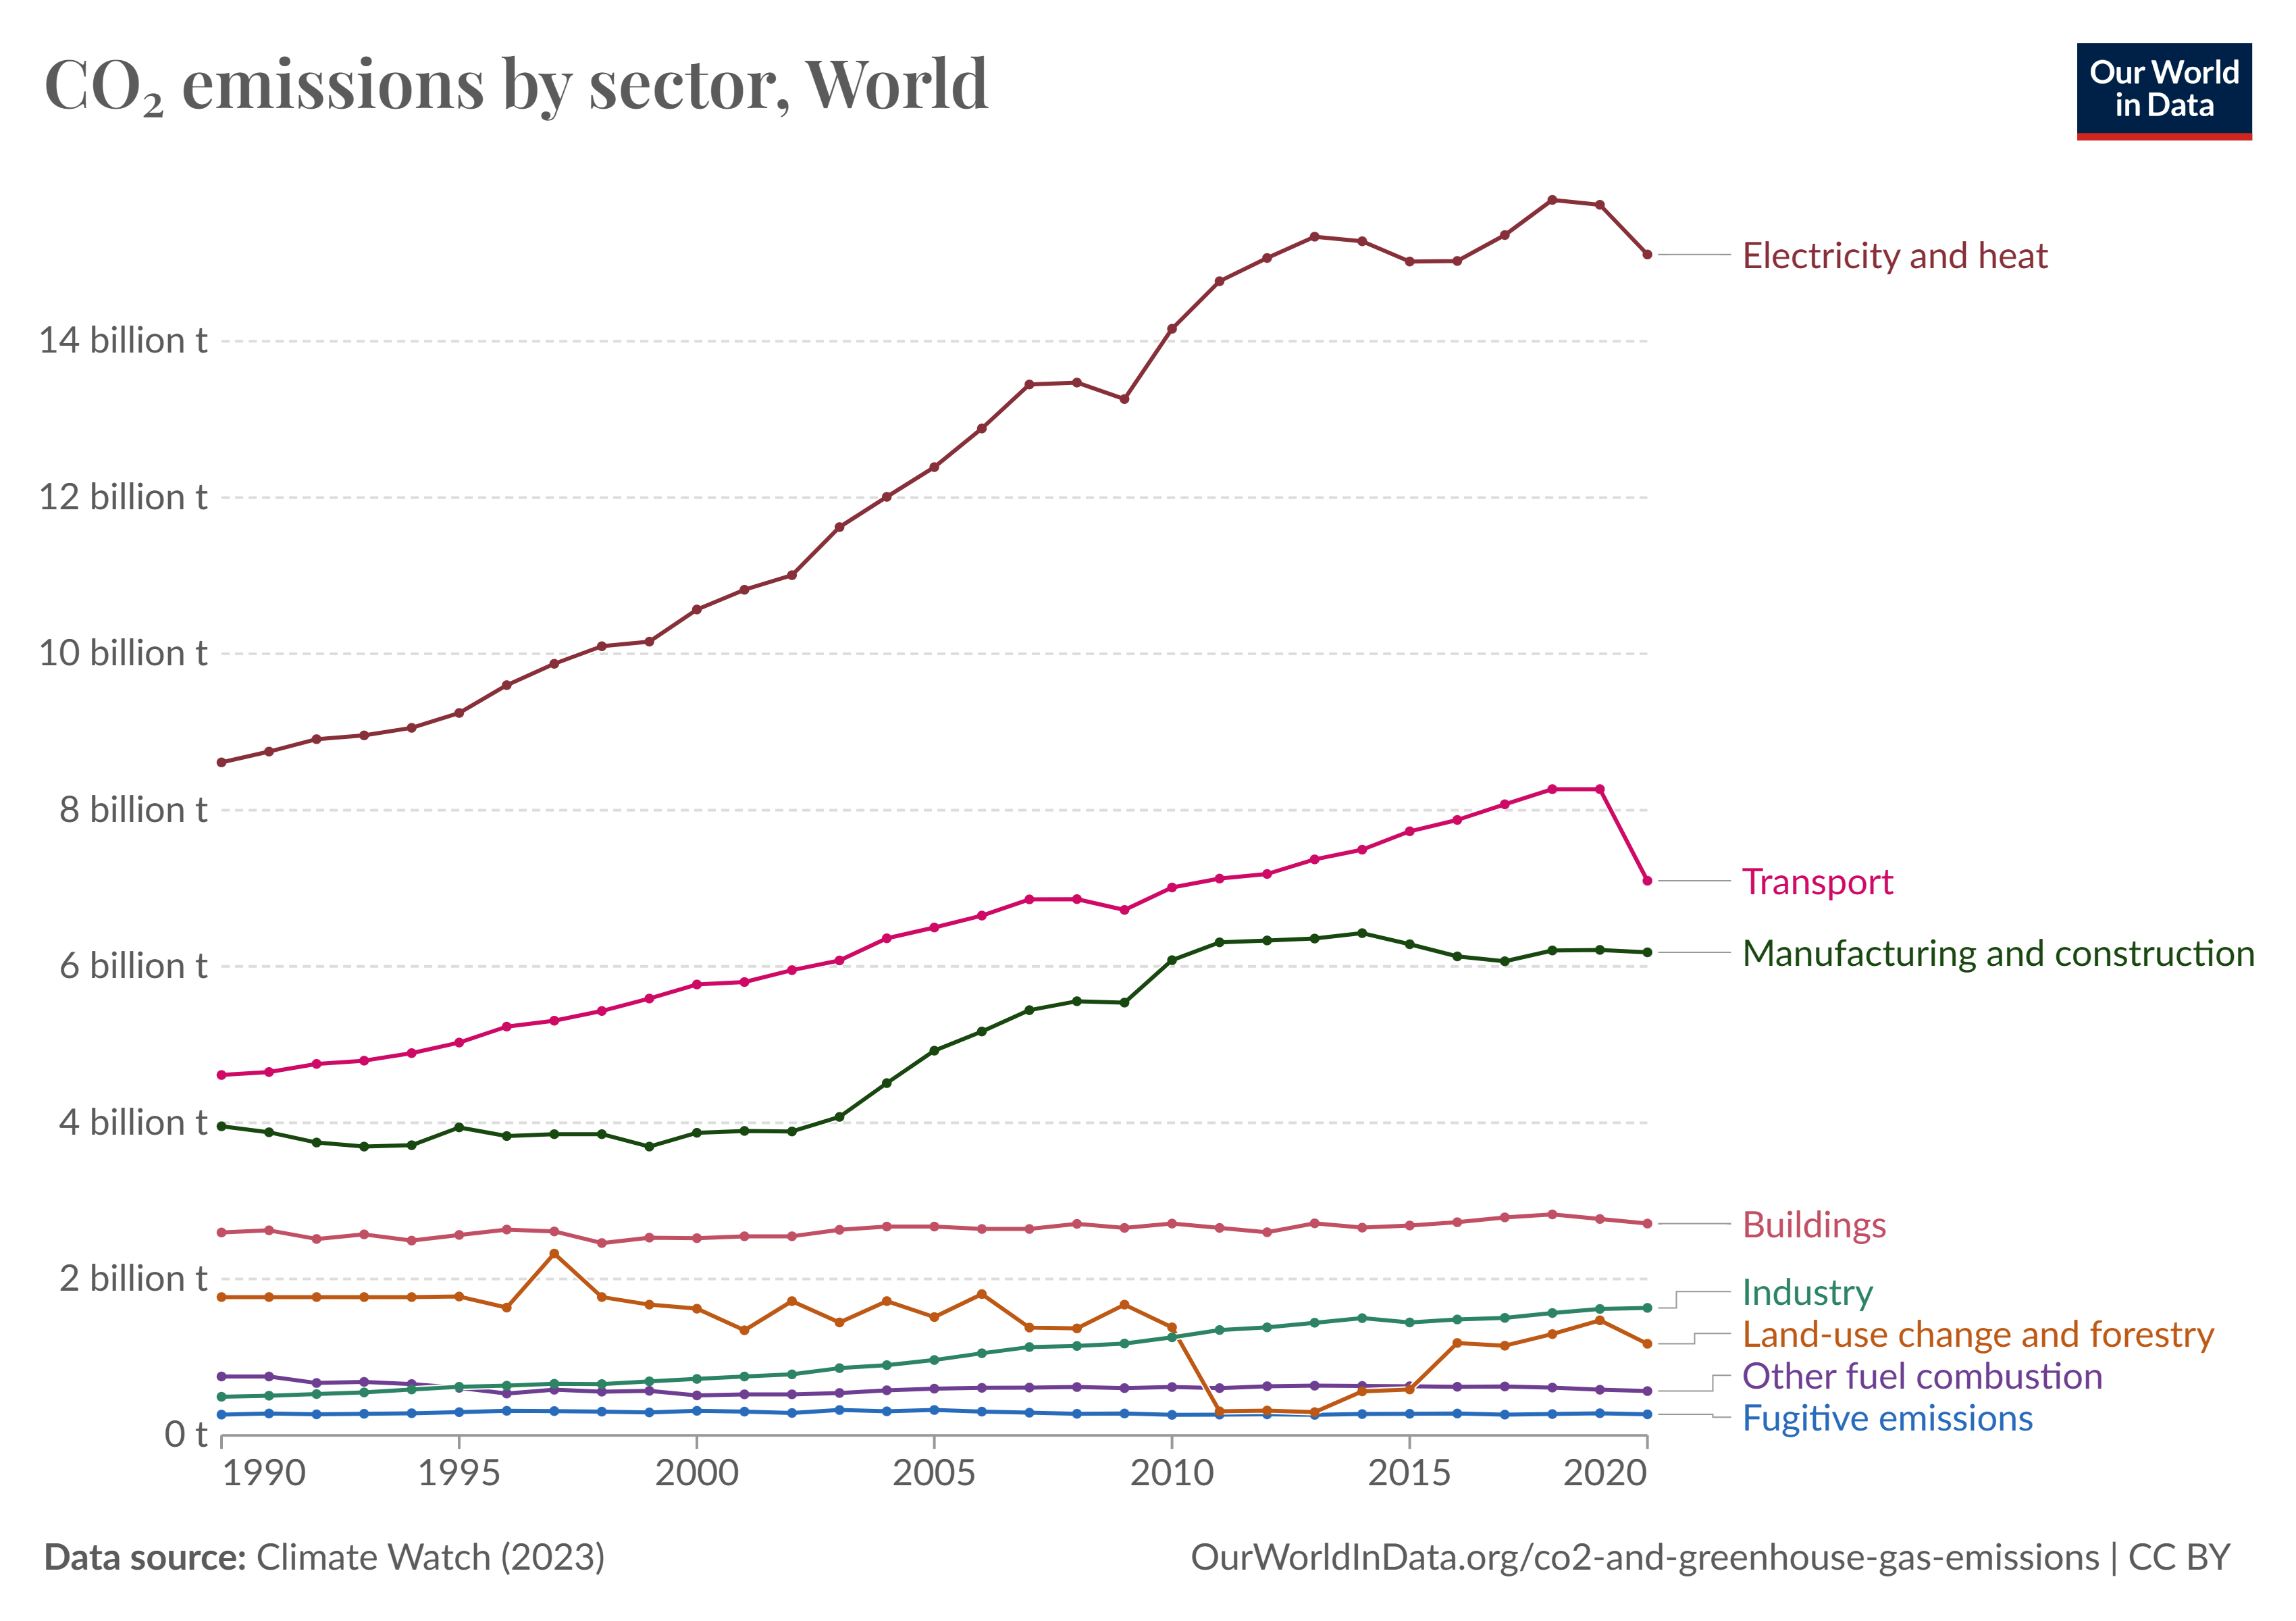
\includegraphics[width=0.8\textwidth]{img/co-emissions-by-sector.png}
    \caption{$\mathrm{CO_2}$ emission by sector\cite{owid-emissions-by-sector}. Transportation is the second-largest source.}
    \label{fig:co2_emission_by_sector}
\end{figure}

\begin{table}[H]
    \centering
    \begin{tabular}{|l|l|l|l|}
        \hline
        ~                          & \textbf{Liquid Ammonia} & \textbf{Gasoline} & \textbf{Diesel} \\
        \hline
        Volumetric [$GJ m^{-3}$]   & 11.38                   & 30.6              & 37.2            \\
        Gravimetric [$MJ Kg^{-1}$] & 18.65                   & 43.6              & 44.8            \\
        \hline
    \end{tabular}
    \caption{Energy density of Ammonia compared to traditional fuels\cite{energy-density}.}
    \label{tab:energy_density}
\end{table}
